\section{Motivation}

%%%%%%%%%%%%%%%%%%%%%%%%%%%%%%%%%%%%%%%%%%%%%%%%%%%%%%%%%%%%%%%%%%%%%%%%%
%%%%%%%%%%%%%%%%%%%%%%%%%%%%%%%%%%%%%%%%%%%%%%%%%%%%%%%%%%%%%%%%%%%%%%%%%
%%%%%%%%%%%%%%%%%%%%%%%%%%%%%%%%%%%%%%%%%%%%%%%%%%%%%%%%%%%%%%%%%%%%%%%%%

\subsection{Arritmia}

%%%%%%%%%%%%%%%%%%%%%%%%%%%%%%%%%%%%%%%%%%%%%%%%%%%%%%%%%%%%%%%%%%%%%%%%%


\begin{frame}
    \begin{center} 
        %\vspace{-2.5cm}
        {\Large \color{TurkishRose}\textbf{\textit{¿Qué es la arritmia?}}} 
    \end{center}
    \pause
     \begin{columns}
        \column{0.5\textwidth}\centering
        Trastorno de la frecuencia (ritmo) cardíaca.
        \begin{itemize}
            \item Taquicardia
            \item Bradicardia
            \item {\color{TurkishRose}\textbf{Fibrilación Auricular}}
        \end{itemize}
        
        \column{0.5\textwidth}\centering
        \begin{figure}
            \centering
            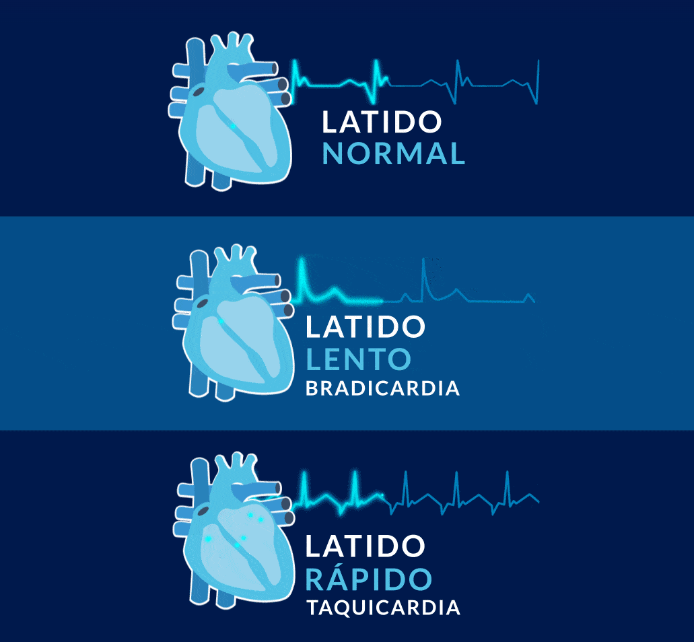
\includegraphics[width=1\textwidth]{Images/arritmia.png}
            \caption{\href{https://cuidandotucorazon.com/wp-content/uploads/2019/07/latido-normal-lento-rapido.gif}{Fuente}}
        \end{figure}
    \end{columns}
    
    
\end{frame}



%%%%%%%%%%%%%%%%%%%%%%%%%%%%%%%%%%%%%%%%%%%%%%%%%%%%%%%%%%%%%%%%%%%%%%%%%
\begin{frame}

   \begin{center}
        \vspace{0cm}
       {\Large \color{TurkishRose}\textbf{\textit{¿Es peligrosa?}}} 
   \end{center}
   
   \pause
   
    \begin{columns}
        \column{0.5\textwidth}\centering
        {\hspace{-2cm}Por lo general...}\\
            \begin{itemize}
                \item Depende del tipo de arritmia.
                \item Hay algunas que no.
                \item Pero si es una fibrilación auricular, entonces sí.
            \end{itemize}
        \column{0.5\textwidth}\centering
            \begin{figure}
                \centering
                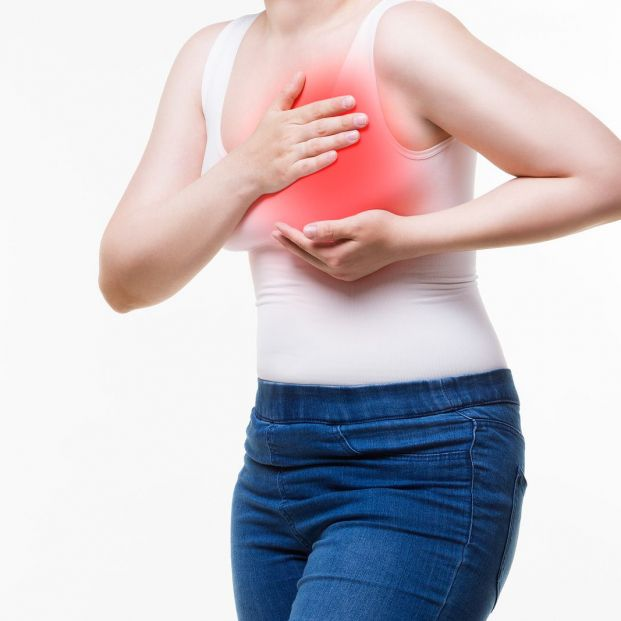
\includegraphics[width=1\linewidth]{Images/arritmia2.png}
                \caption{\href{https://www.65ymas.com/uploads/s1/92/58/1/fibrilacion-auricular_1_621x621.jpeg}{Fuente}}
            \end{figure}
    \end{columns}
\end{frame} 


%%%%%%%%%%%%%%%%%%%%%%%%%%%%%%%%%%%%%%%%%%%%%%%%%%%%%%%%%%%%%%%%%%%%%%%%%

\begin{frame}
    \begin{center}
                %\vspace{1.9cm}
                {\Large \color{TurkishRose}\textbf{\textit{¿Cómo de peligrosa es la fibrilación auricular?}}} 
    \end{center}
    \pause
    \begin{columns}
        
        \column{0.5\textwidth}\centering
            \vspace{-2cm}
            \begin{itemize}
                \item Afecta al $1-2\%$ de la población.
                \item No entiende de géneros.
                \item Su incidencia aumenta con la edad.
                \item En los próximos 30 años su incidencia aumentará el triple.
                \item Asociada a una alta tasa de mortandad y morbilidad.
            \end{itemize}
        \pause
        \column{0.5\textwidth}\centering
            {\hspace{-2.5cm}Puede causar} \\
            \begin{itemize}
                \item Cansancio y fatiga
                \item Accidente cerebrovascular.
                \item Infarto cerebral
                \item Y en el peor de los casos...
            \end{itemize}
            \pause 
            \begin{figure}
                \centering
                \includegraphics[width=0.8\textwidth]{Images/death2.png}
                \caption{\href{https://javieres.com/wp-content/uploads/2022/04/LOGOERDGERTF.png}{Fuente}}
            \end{figure}

            
    \end{columns}
\end{frame}

%%%%%%%%%%%%%%%%%%%%%%%%%%%%%%%%%%%%%%%%%%%%%%%%%%%%%%%%%%%%%%%%%%%%%%%%%

%\begin{frame}
%\begin{center}
%    {\vspace{-1cm} \Large \color{TurkishRose}\textbf{\textit{¿Alguna buena noticia?}}} \\
%\end{center}
%    \pause
%    \begin{center}
%        No hay que preocuparse si... \\
%        \pause
%        \vspace{1cm}
%            \begin{itemize}
%                \setlength\itemsep{1.5em}
%                \item {\color{TurkishRose}\textbf{\textit{es detectada a tiempo}}} \\
%                \pause
%                \item es tratada adecuadamente por profesionales. \\
%                \pause
%                \item se acude periódicamente a revisiones. \\
%            \end{itemize}
%        
%    \end{center}
%\end{frame}

%%%%%%%%%%%%%%%%%%%%%%%%%%%%%%%%%%%%%%%%%%%%%%%%%%%%%%%%%%%%%%%%%%%%%%%%%


\begin{frame}
    \begin{center}
        {\vspace{-1cm} \Large \color{TurkishRose}\textbf{\textit{¿Cómo la detectamos?}}} \\
    \end{center}

    \pause
    \begin{center}
    \vspace{1cm}
        \begin{itemize}
            \setlength\itemsep{1em}
            \item De eso trata este proyecto. \\
            \pause
            \item Primeramente, vayamos a los fundamentos de todo... \pause {\color{TurkishRose} \textit{las matemáticas}}
            \pause
            \item  Después, a las técnicas de aprendizaje profundo.
            \pause 
            \item Y por último, nos enfrentamos a las fibrilaciones auriculares.
        \end{itemize}
    \end{center}
    
\end{frame}


